\chapter{Análisis de riesgos}
\setlength{\parindent}{2em}
El análisis de riesgos es el proceso que permite la identificación de las amenazas que pueden perjudicar al desarrollo del proyecto y determinar el impacto o grado de perjuicio que pueden ocasionar. Implica analizar las amenazas y vulnerabilidades que puedan darse y se valoran en términos de probabilidad de ocurrencia y gravedad de impacto sobre el proyecto.

\hspace*{2em}A continuación, se establece una escala (de menor a mayor gravedad) para valorar el impacto que causarían los riesgos que se describen a continuación:
	\begin{itemize}
		\item \emph{\textbf{Muy grave:}} De consecuencias fatales para el desarrollo del proyecto, requeriría replantearse, incluso, si merece la pena continuar con el proyecto.
		\item \emph{\textbf{Grave:}} Problemas que podrían imposibilitar terminar el proyecto en el plazo previsto. Requeriría realizar una profunda re planificación ampliando el número de horas a dedicar o reduciendo el trabajo a realizar.
		\item \emph{\textbf{Perjudicial:}} Pequeños retrasos relativamente sencillos de solventar, aunque pueden resultar peligrosos si no se identifican y subsanan a tiempo.
	\end{itemize}


\begin{figure}[H]
	\centering
	
\includegraphics[width=0.6\linewidth]{figuras/riesgo}
	\label{fig:riesgo}
\end{figure}

\section{Fichas de riesgo}

\hspace*{2em}Los posibles riesgos comunes que se tienen en cuenta en la realización del proyecto los siguientes:\\
	
 	\begin{shaded}
		\underline{\textbf{Elección equivocada de las herramientas de trabajo:}}
		\begin{flushleft}
			\textbf{Descripción:} Es posible que con alguna de las tecnologías elegidas no sea posible cumplir los objetivos planteados o dar a la aplicación la funcionalidad deseada.\\
			\textbf{Probabilidad:} 5\\
			\textbf{Alcance:} Muy grave, ya que supondría replantear por completo el proyecto.\\
			\textbf{Medidas preventivas:} no es necesario adoptar medidas preventivas ya que por requisitos tecnológicos las herramientas de trabajo estaban muy definidas.
		\end{flushleft}	
	\end{shaded}
	
	
	\begin{shaded}
		\underline{\textbf{Desconocimiento del software elegido:}}
		\begin{flushleft}	
			\textbf{Descripción:}  En este proyecto se van a usar varias herramientas con las que el desarrollador no está nada familiarizado y esto podría ocasionar retrasos a la hora de realizar la aplicación.\\
			\textbf{Probabilidad:} 90\\
			\textbf{Alcance:} Perjudicial, impediría avanzar en el tiempo estimado.\\
			\textbf{Medidas preventivas:} no es necesario adoptar medidas preventivas ya que el desarrollador conoce las herramientas y tiene experiencia con las mismas.
		\end{flushleft}			
	\end{shaded}
	
	\begin{shaded}
		\underline{\textbf{Estancamiento en la codificación:}}
		\begin{flushleft}	
			\textbf{Descripción:}  Podría llegar a darse algún problema de difícil solución que paralizaría momentáneamente el avance del proyecto.\\
			\textbf{Probabilidad:} 20\\
			\textbf{Alcance:} Perjudicial, impediría avanzar en el tiempo estimado.\\
			\textbf{Medidas preventivas:} Medidas preventivas: Se Mantiene un seguimiento por medio de metodologías ágiles, así pues, el cliente sabe en todo momento cómo va el desarrollo del trabajo a través de los Sprints  
		\end{flushleft}			
	\end{shaded}
\clearpage	
	\begin{shaded}
		\underline{\textbf{Pérdida de los datos por fallo del hardware o software maligno:}}
		\begin{flushleft}	
			\textbf{Descripción:} Debido a un virus o a un fallo en el disco duro del ordenador en el que se desarrolla el proyecto se podrían perder todos los datos.\\
			\textbf{Probabilidad:} 10\\
			\textbf{Alcance:} Muy grave, pues supondría empezar de cero.\\
			\textbf{Medidas preventivas:} Se ha implantado un sistema de control de versiones (git) y una copia de seguridad del entorno de desarrollo, ademas de herramientas anti-virus y anti-malware. 
		\end{flushleft}			
	\end{shaded}
		
	\begin{shaded}
		\underline{\textbf{Problema con los recursos materiales:}}
		\begin{flushleft}	
			\textbf{Descripción:} El coste material y del software no puede ser asumido.\\
			\textbf{Probabilidad:} 10\\
			\textbf{Alcance:} Perjudicial, ya que retrasarían el proyecto de una forma indefinida.\\
			\textbf{Medidas preventivas:}  El material adicional necesario es proporcionado por la pyme en modelo de préstamo. Las licencias de desarrollo de los sistemas elegidos son de libre uso y distribución.  
		\end{flushleft}			
	\end{shaded}

	\begin{shaded}
		\underline{\textbf{Baja del desarrollador de la aplicación:}}
		\begin{flushleft}	
			\textbf{Descripción:} Podría suceder que, por enfermedad o accidente, el desarrollador del proyecto quede incapacitado durante una temporada.\\
			\textbf{Probabilidad:} 5\\
			\textbf{Alcance:} Perjudicial, puesto que impide la realización del proyecto.\\
			\textbf{Medidas preventivas:} No aplicables.
		\end{flushleft}			
	\end{shaded}
	
\chapter{Planificación del tiempo del proyecto}

\hspace*{2em}Este apartado describe la estructura de descomposición del trabajo utilizada en la realización de la aplicación, las fases, tareas y entregables del proyecto, así como la agenda de trabajo y los recursos materiales empleados. Hay que tener en cuenta que vamos a utilizar una metodología de gestión ágil.\cite{scrum}
\section{Descripción General de la Metodología}
\subsection{Fundamentación}

Las principales razones del uso de un ciclo de desarrollo iterativo e incremental de tipo SCRUM para la ejecución de este proyecto son:
\begin{itemize}
	\item Sistema modular. Las características del sistema Intraza permiten desarrollar una base funcional mínima y sobre ella ir incrementando las funcionalidades o modificando el comportamiento o apariencia de las ya implementadas.
	\item Entregas frecuentes y continuas al cliente de los módulos terminados, de forma que puede disponer de una funcionalidad básica en un tiempo mínimo y a partir de ahí un incremento y mejora continua del sistema.
	\begin{itemize}
		\item 	Previsible inestabilidad de requisitos.
		\item 	Es posible que el sistema incorpore más funcionalidades de las inicialmente identificadas.
		\item 	Es posible que durante la ejecución del proyecto se altere el orden en el que se desean recibir los módulos o historias de usuario terminadas.
		\item 	Al cliente le resulta difícil precisar la dimensión completa del sistema, y su crecimiento puede continuarse en el tiempo suspenderse o detenerse.
	\end{itemize}
\end{itemize}

\subsection{Artefactos}
\begin{itemize}
	\item	Documentos
	\begin{itemize}
		\item Pila de producto 
		\item Pila de Sprint 
	\end{itemize}
	\item Gráficas para registro y seguimiento del avance.
	\begin{itemize}
		\item Gráfica de producto 
		\item	Gráfica de avance 
	\end{itemize}
	\item Comunicación Reunión de inicio de Sprint
	\begin{itemize}
		\item	Reunión técnica diaria
		\item	Reunión de cierre de Sprint y entrega del incremento
	\end{itemize}
\end{itemize}

\subsubsection{Pila de producto}
\hspace*{2em}Es el equivalente a los requisitos del sistema o del usuario en esta metodología.  El gestor de producto puede recabar las consultas y asesoramiento que pueda necesitar para su redacción y gestión durante el proyecto al SCRUM MASTER de este proyecto.

\begin{itemize}
	\item Responsabilidades del gestor de producto
	\begin{itemize}
		\item Registro en la lista de pila del producto de las historias de usuario que definen el sistema.
 		\item Mantenimiento actualizado de la pila del producto en todo momento durante la ejecución del proyecto.
 		\begin{itemize}
			\item Orden en el que desea recibir terminada cada historia de usuario.
			\item Incorporación / eliminación /modificaciones de las historias o de su orden de prioridad.
			\item Disponibilidad: mantiene directamente la pizarra o intranet o medios de comunicación.
		\end{itemize}
	\end{itemize}
	\item Responsabilidades del SCRUM MASTER
	\begin{itemize}
		\item	Supervisión de la pila de producto, y comunicación con el gestor del producto para pedirle aclaración de las dudas que pueda tener, o asesorarle para la subsanación de las deficiencias que observe.
	\end{itemize}
	\item Responsabilidades del equipo técnico
	\begin{itemize}
		\item	Conocimiento y comprensión actualizado de la pila del producto. 
		\item	Resolución de dudas o comunicación de sugerencias con gestor de producto / SCRUM MASTER.
	\end{itemize}	
	\item Responsabilidades del resto de implicados
	\begin{itemize}
		\item Conocimiento y comprensión actualizado de la pila del producto.
		\item Resolución de dudas o comunicación de sugerencias con gestor de producto o SCRUM MASTER.
	\end{itemize}
\end{itemize}	

\subsubsection{Pila del Sprint}
\hspace*{2em}Es el documento de registro de los requisitos detallados o tareas que va a desarrollar el equipo técnico en la iteración (actual o que está preparándose para comenzar)
	
	\begin{itemize}
		\item Responsabilidades del gestor de producto
		\begin{itemize}
			\item Presencia en las reuniones en las que el equipo elabora la pila del Sprint. Resolución de dudas sobre las historias de usuario que se descomponen en la pila del Sprint.
		\end{itemize}	 
		\item Responsabilidades del SCRUM MASTER
		\begin{itemize}
			\item	Supervisión y asesoría en la elaboración de la pila del Sprint.
		\end{itemize}	
		\item Responsabilidades del equipo técnico
		\begin{itemize}
			\item	Elaboración de la pila del Sprint 
			\item	Resolución de dudas o comunicación de sugerencias sobre las historias de usuario con el gestor del producto.
		\end{itemize}
	\end{itemize}	

\subsubsection{Sprint}
\hspace*{2em}Cada una de las iteraciones del ciclo de vida iterativo SCRUM. La duración de cada Sprint es en el caso que nos ocupa 2 semanas de 5 días laborables cada una.

\subsubsection{Gráfica de producto (Burn Up)}
\hspace*{2em}Representación gráfica del plan de producto previsto por el gestor de producto. Es una gráfica que representa los temas o epics del sistema en el orden que se desean, y el tiempo en el que se prevé su ejecución. 

	\begin{itemize}
		\item Responsabilidades del gestor de producto
		\begin{itemize}
			\item	Confección.
			\item	Mantenimiento actualizado en todo momento durante la ejecución del proyecto.
			\item	Orden en el que desea disponer de los temas o “epics” del sistema, e hitos del producto (versiones). 
			\item	Incorporación / eliminación /modificaciones de los temas, de su orden de prioridad, estimaciones o hitos.
			\item	Disponibilidad:  mantiene directamente la pizarra o intranet o medios de comunicación.
		\end{itemize}
		\item Responsabilidades del SCRUM MASTER
		\begin{itemize}
			\item Supervisión del gráfico de producto, y comunicación con el gestor del producto para pedirle aclaración de las dudas que pueda tener, o asesorarle para la subsanación de las deficiencias que observe.
		\end{itemize}		
		\item Responsabilidades del equipo técnico
		\begin{itemize}
			\item	Conocimiento y comprensión actualizado del plan del producto. 
			\item	Resolución de dudas o comunicación de sugerencias con gestor de producto o SCRUM MASTER.
		\end{itemize}	
		\item Responsabilidades del resto de implicados
		\begin{itemize}
			\item	Conocimiento y comprensión actualizado del plan de producto.
			\item	Resolución de dudas o comunicación de sugerencias con gestor de producto o SCRUM MASTER.
		\end{itemize}	
	\end{itemize}

\subsubsection{Gráfica de avance (Burn Down)}

\hspace*{2em}Gráfico que muestra el estado de avance del trabajo del Sprint en curso.
	\begin{itemize}
		\item Responsabilidades del gestor de producto
		\begin{itemize}
			\item Sin responsabilidades específicas, más allá de mantenerse regularmente informado del avance del Sprint y disponible para atender decisiones para la resolución de opciones en Sprints sobre-valorados o infravalorados (la gráfica de avance predice una entrega anterior o posterior a la fecha prevista)
		\end{itemize}
		\item Responsabilidades del SCRUM MASTER
		\begin{itemize}
			\item Supervisión de la actualización diaria por parte del equipo.
		\end{itemize}		
		\item responsabilidades del equipo técnico
		\begin{itemize}
			\item Actualización diaria del gráfico de avance.
		\end{itemize}
	\end{itemize}	

\subsubsection{Reunión de inicio de Sprint}

\hspace*{2em}Reunión para determinar las funcionalidades o historias de usuario que se van a incluir en el próximo incremento.

	\begin{itemize}
		\item Responsabilidades del gestor de producto
		\begin{itemize}
			\item Asistencia a la reunión.
			\item	Exposición y explicación de las historias que necesita para la próxima iteración y posibles restricciones de fechas que pudiera tener.
		\end{itemize}
		\item Responsabilidades del SCRUM MASTER
		\begin{itemize}
			\item Moderación de la reunión
		\end{itemize}
		\item Responsabilidades del equipo técnico
		\begin{itemize}
			\item	Confección de la pila del Sprint.
			\item	Auto-asignación del trabajo.
		\end{itemize}
	\end{itemize}

\subsubsection{Reunión técnica diaria}

\hspace*{2em}Puesta en común diaria del equipo con presencia del Coordinador del proyecto o SCRUM MASTER de duración máxima de 10 minutos.

	\begin{itemize}
		\item Responsabilidades del SCRUM MASTER
		\begin{itemize}
			\item Supervisión de la reunión y anotación de las necesidades o impedimentos que pueda detectar el equipo.
			\item Gestión para la solución de las necesidades o impedimentos detectados por el equipo.
		\end{itemize}
		\item Responsabilidades del equipo técnico
		\begin{itemize}
			\item Comunicación individual del trabajo realizado el día anterior y el previsto para día actual.
			\item Actualización individual del trabajo pendiente.
			\item Actualización del gráfico de avance para reflejar el estado de avance.
			\item Notificación de necesidades o impedimentos previstos u ocurridos para realizar las tareas asignadas.
		\end{itemize}
	\end{itemize}

\subsubsection{Reunión de cierre de Sprint y entrega del incremento}

\hspace*{2em}Reunión para probar y entregar el incremento al gestor del producto.

Características.
	\begin{itemize}
		\item Prácticas: sobre el producto terminado, no sobre simulaciones o imágenes.
		\item De tiempo acotado máximo de 2 horas.
	\end{itemize}

	\begin{itemize}
		\item Responsabilidades del gestor de producto
		\begin{itemize}
			\item Asistencia a la reunión.
			\item Recepción del producto o presentación de reparos.
		\end{itemize}
		\item Responsabilidades del SCRUM MASTER
		\begin{itemize}
			\item Moderación de la reunión
		\end{itemize}	
		\item Responsabilidades del equipo técnico
		\begin{itemize}
			\item	Presentación del incremento.
		\end{itemize}
	\end{itemize}


\begin{figure}[H]
	\centering
	\fcolorbox{black}{white}{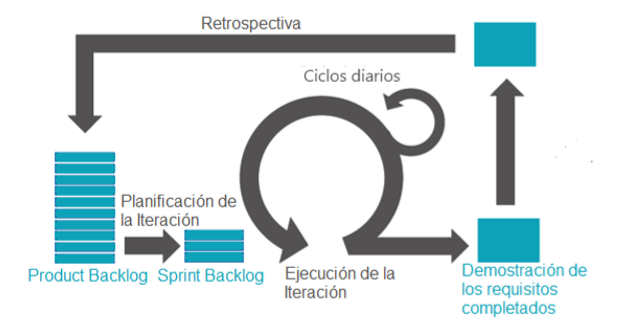
\includegraphics[width=0.95\linewidth]{figuras/ciclo}}
	\caption[Ciclo]{Ciclo del proyecto}
	\label{fig:ciclo}
\end{figure}


\subsection{Particularidades de este proyecto}
\hspace*{2em}En este proyecto la figura del SCRUM MASTER y el equipo técnico recaen sobre una sola persona.  Bajo esta particularidad desaparecen las reuniones técnicas diarias.
La figura del gestor del producto viene dada por un contacto con la empresa cliente. Las reuniones de comienzo del Sprint y final de Sprint se realizan bajo herramientas de videoconferencia, y teamviewer.	\\ 









